\documentclass[a4paper,11pt]{article}
\usepackage[margin=3cm]{geometry}
\linespread{1.25}

\usepackage[T1]{fontenc}
\usepackage[utf8]{inputenc}
% \usepackage[swedish]{babel}
% \usepackage{fontspec}
% \setmainfont{Linux Libertine O}
\usepackage{lmodern}
\usepackage{graphicx}
\usepackage{float}
\usepackage{subfig}

\usepackage{fancyhdr}
\pagestyle{fancy}
\renewcommand{\headrulewidth}{ 1.0pt }
\renewcommand{\footrulewidth}{ 0.4pt }
\fancyhead{} % clear all headers
\fancyfoot{} % clear all footers

% E:even page, O:odd page, L:left, C:center, R:right
%\fancyhead[LE,RO]{\thepage}
%\fancyfoot[C]  {Albert Einstein, 2009}

\fancyhead[L]{DH2323 (DGI17) Lab 3}
\fancyhead[R]{Mikael Forsberg, Robin Gunning}
\fancyfoot[C]{\thepage}

\begin{document}
\title{\vspace{-2cm} Lab 3: Rasterisation\\ \small DH2323 (DGI17)\\ KTH Royal Institute of Technology}
\author{Mikael Forsberg <miforsb@kth.se>\\ Robin Gunning <rgunning@kth.se>}
\maketitle

\vspace{-1.25cm}

\section*{Overview}
We completed all the given tasks and added camera pitch, mouse control and backface culling.

\section*{Controls}
\begin{itemize}
\item Mouse motion: camera pitch and yaw
\item Arrow keys: camera pitch and yaw
\item WASD+(Q,E): camera movement
\item 1,2,3,4,5,6: light movement
\end{itemize}

\section*{Transformations}
As we've already done the pinhole camera in labs 1 and 2 it was relatively easy to implement again.
The transformations were easy to implement as all the required formulas were presented in an easy-to-understand
manner. 

\section*{Drawing Points}
Drawing the points was essentially the same problem that we had already dealt with in the
starfield part of lab 1.

\begin{figure}[H]
\begin{center}
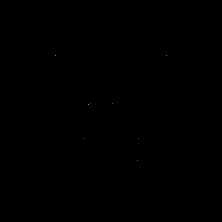
\includegraphics[width=5cm]{dots.jpg}
\caption{The vertices of the Cornell box}
\end{center}
\end{figure}
\vspace{-1.5cm}

\bigskip
\bigskip
\noindent You can ''clearly'' see that the points in the picture represent the Cornell box.

\section*{FOV in theory and practice}
This section aims to answer the question regarding FOV posed in the lab instructions.

\begin{figure}[H]
\begin{center}
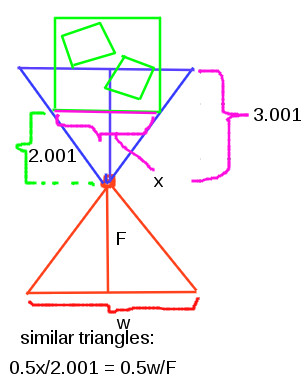
\includegraphics[width=5cm]{camerapos.jpg}
\caption{FOV calculation diagram}
\end{center}
\end{figure}

\noindent Let $F$, $w$ and $h$ be the same number, say $F = w = h = 320$. Let the camera be
positioned at $(0,0,-3)$ and have all angles of rotation at zero. A point on the vertical midpoint
of the front edge of the left wall of the Cornell box is located at $(-1,0,-1)$. The corresponding
right point is located at $(1,0,-1)$. Translating to camera space the left point is located at
$(-1,0,-1) - (0,0,-3) = (-1,0,2)$ and the right point at $(1,0,-1) - (0,0,-3) = (1,0,2)$
Projecting the left point onto screen space we get $x' = F*x/z + w/2 = 320*(-1/2) + 320/2 = 0$ and
for the right point we get $x' = F*x/z + w/2 = 320*(1/2) + 320/2 = 320$ meaning the two points are situated
at the exact horizontal extremes of the screen. An analogous result can be shown for a pair of points on the
midpoints of the front edges of the floor and roof of the box.

From the diagram (Figure 2) we see that at a distance of $2.001$ from the pinhole of the camera the
maximum difference in $x$ that can fit on the screen (assuming $F = w$) is precisely $2.001$, which
means that the entire Cornell box will be visible since it happens to have a side width of $2$.

\section*{Drawing Edges}
To draw the edges we used the linear interpolation learned from lab 1.
To fix the issue with vertices being behind the camera we added a form of ''fake'' clipping
by looking at the camera space z-coordinates of triangle vertices and skipping the entire
triangle as soon as any vertex is found located at $z < 1$. This is not a good solution since it
causes triangles to ''pop out of existence'' when one or more of its vertices ends up
too close to the camera, but we believe it is better than nothing.

Implementing camera movement and rotation was easy as we had already done so for lab 2.

\begin{figure}[H]
\begin{center}
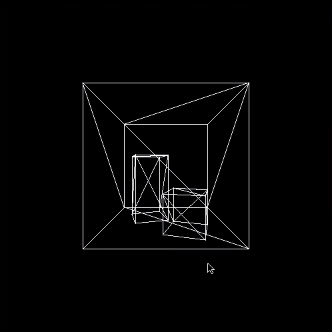
\includegraphics[width=7cm]{wire.jpg}
\caption{Wireframe image of the Cornell box}
\end{center}
\end{figure}
\vspace{-0.5cm}

\section*{Filled Triangles}
We first computed how tall the triangle will be ($\Delta y$) to get the number of rows needed. 
Then we walked each edge (or so we thought) of the triangle computing $x_{min}$ and $x_{max}$ for
every row. Finally we drew the rows to the screen in the color of said triangle.

As hinted to we had an issue with missing one of the edges (one of the vertex pairs) in the loop that was
supposed to walk all the edges.

\begin{figure}[H]
    \centering
    \subfloat[Missing an edge]{{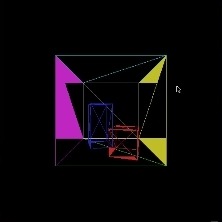
\includegraphics[width=5cm]{fillerror2.jpg} }}
    \qquad
    \subfloat[All edges included]{{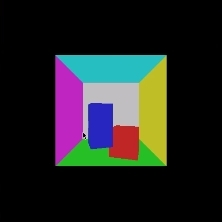
\includegraphics[width=5cm]{fill.jpg} }}
    \caption{Drawing filled triangles}
\end{figure}

\section*{Depth Buffer}
The depth buffer was pretty straightforward to understand and implement. However, implementing 
the new struct Pixel and changing almost every function we had already created was time consuming and
frustrating. The reason for using $1/z$ is still pretty mysterious, as also mentioned below.

\section*{Illumination}
The per-vertex illumination was similar to the bilinear interpolation done in lab 1.
The effect of per-vertex illumination was itself quite reminiscent of the way games tended to look 
running on early 3D-acceleration hardware in the late 1990's.
The switch to per-pixel illumination mainly consisted of adding even more elements to the interpolation 
function and not forgetting to copy them in when computing the rows for drawing.

We did have an art-generating issue at some stage in implementing lighting (see Figure 5), but neither
of us remembers what caused it.

Making the per-pixel lighting be perspective-correct again involved the somewhat mysterious maths trick of 
premultiplying values by $1/z$ in order to be able to interpolate them in screen-space and later 
restore them by dividing by $1/z$. We still don't really have an intuitive grasp on why this works.

\begin{figure}[H]
\begin{center}
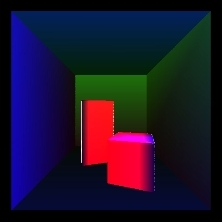
\includegraphics[width=7cm]{lighterror.jpg}
\caption{Some problem with lighting}
\end{center}
\end{figure}
\vspace{-0.5cm}

\section*{Result}

\begin{figure}[H]
\begin{center}
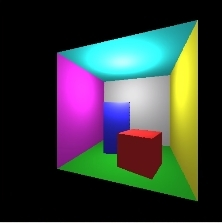
\includegraphics[width=7cm]{light.jpg}
\caption{Final result}
\end{center}
\end{figure}
\vspace{-0.5cm}

\section*{Bonus additions}
\subsection*{Camera pitch}
We added support for camera pitch by extending the camera code from lab 2 using the standard
matrix for rotation about the x-axis. The two rotation matrices are multiplied together to create a
final rotation matrix. We do not allow the camera heading to be affected by the pitch, and so we extract
the heading before performing the matrix multiplication.

\subsection*{Camera control with mouse}
We added support for controlling the camera pitch and yaw using the mouse, using the suggested
\texttt{SDL\_GetRelativeMouseState} function. This was fairly straightforward except for an issue
where the function returned very large readings immediately at the start of the program. We fixed this
by ignoring the mouse during the first 500 ticks (by \texttt{SDL\_GetTicks}) of runtime.

\subsection*{Backface culling}
We implemented the simplest possible form of backface culling by skipping any triangles
where the angle between the surface normal of the triangle and a vector from the triangle
to the camera position exceeds 90 degrees. Since we don't take the camera heading and FOV
into account we are not able to cull triangles that are behind the camera.

\section*{Contributions}
All of the hard requirements were completed as a joint effort. Mikael implemented the bonus
additions mentioned above (camera pitch, mouse controls and backface culling).

\end{document}
